%%%%%%%%%%%%%%%%%%%%%%% file template.tex %%%%%%%%%%%%%%%%%%%%%%%%%
%
% This is a general template file for the LaTeX package SVJour3
% for Springer journals.          Springer Heidelberg 2010/09/16
%
% Copy it to a new file with a new name and use it as the basis
% for your article. Delete % signs as needed.
%
% This template includes a few options for different layouts and
% content for various journals. Please consult a previous issue of
% your journal as needed.
%
%%%%%%%%%%%%%%%%%%%%%%%%%%%%%%%%%%%%%%%%%%%%%%%%%%%%%%%%%%%%%%%%%%%

\RequirePackage{fix-cm}
%
%\documentclass{svjour3}                     % onecolumn (standard format)
%\documentclass[smallcondensed]{svjour3}     % onecolumn (ditto)
\documentclass[smallextended]{svjour3}       % onecolumn (second format)
%\documentclass[twocolumn]{svjour3}          % twocolumn
%
\smartqed  % flush right qed marks, e.g. at end of proof
%
\usepackage{graphicx}
\usepackage{natbib}
%
% \usepackage{mathptmx}      % use Times fonts if available on your TeX system
%
% insert here the call for the packages your document requires
%\usepackage{latexsym}
% etc.
%
% please place your own definitions here and don't use \def but
% \newcommand{}{}
%
% Insert the name of "your journal" with
\journalname{Attention, Perception, \& Psychophysics}
%
\begin{document}

\title{Replicating the visual search visualisation experiment\thanks{Say thanks to Amelia's grant}}
\subtitle{Do the results stand up? Do they generalise?}

\titlerunning{Short form of title}        % if too long for running head

\author{Alasdair D. F. Clarke         \and
        Amelia R. Hunt
}

%\authorrunning{Short form of author list} % if too long for running head

\institute{F. Author \at
              first address \\
              Tel.: +123-45-678910\\
              Fax: +123-45-678910\\
              \email{fauthor@example.com}           %  \\
%             \emph{Present address:} of F. Author  %  if needed
           \and
           S. Author \at
              second address
}

\date{Received: date / Accepted: date}
% The correct dates will be entered by the editor


\maketitle

\begin{abstract}
We propose a replication and generalisation of some striking results on the effect of mental imagery on visual search performance. 
\keywords{mental imagery \and visual attention, \and learning \and visual search \and perception \and open materials}
% \PACS{PACS code1 \and PACS code2 \and more}
% \subclass{MSC code1 \and MSC code2 \and more}
\end{abstract}

%%%%%%%%%%%%%%%%%%%%%%%%%%%%%%%%%%%%%%%%%%%%%%%%%%%%%
\section{Introduction}
\label{sec:intro}
%%%%%%%%%%%%%%%%%%%%%%%%%%%%%%%%%%%%%%%%%%%%%%%%%%%%%

Mental imagery, also referred to as visualising, is the phenomenon where by a person constructs a mental representation of an image (or activity). This can strongly resemble the experience of perceiving the scene or object (or carrying out an activity), but it occurs when the stimulus is not actually present. It has been used as a training exercise for athletes \citep{??}. One hypothesis is that imagery has training benefits as it improves motor control \citep{crammond1997} and visuo-motor coordination \citep{binder2014}.

An intriguing hypothesis is these training effects can come about to by improving low level visual perception and attention, leading to the task-relevant information in the visual input to be processed more efficiently. This possibility was recently explored by \cite{reinhart2015} who found evidence that attentional mechanisms can be effectively trained to select target objects. What's more, the surprisingly found that the effect from visualisation training was stronger (shorter reaction times) than the effect of practising the task itself. They used a \ldots

We found this result particularly striking. We propose a replication of the original study by \cite{reinhart2015}, although will only test the behavioural part of the results. This allows us to use a slightly simplified stimuli design (no need to take lateral what's it effects into account). We also plan a second experiment using a more traditional visual search paradigm in which the observer's task is to determine whether the target is present or absent. This will allow us to explore whether this visualisation-benefit can be observed in general visual search tasks, or if it is particular to the stimuli and task used by \cite{reinhart2015}. We will also analyse the data in more depth using linear-mixed-effect models and explore how the visualisation effect related to serial dependency effects \citep{fischer-whitney2014}.


%%%%%%%%%%%%%%%%%%%%%%%%%%%%%%%%%%%%%%%%%%%%%%%%%%%%%
\section{Experiment 1}
\label{sec:exp1}
%%%%%%%%%%%%%%%%%%%%%%%%%%%%%%%%%%%%%%%%%%%%%%%%%%%%%

The aim of this experiment is to directly replicate the visualisation effect in visual search \citep{reinhart2015}. We have made two minor changes to the original paradigm: (i) we have removed the red distracter element used in the original study to control for EEG effects. (ii). We will use runs of length three, four and five, rather than three, five and seven. This was done as runs of longer length are unimportant for testing the critical result: that reaction times for trial three in a run will be faster in the visualise condition than those in the practise condition. 

\subsection{Methods}

\subsubsection{Participants}

30 participants will be recruited via from \ldots from the University of Aberdeen. All participants will have normal or corrected-to-normal vision. 

The sample size of $n=30$ is based on a power analysis for a one-tailed paired $t$-test, with a power of 0.9 and effect size of $d=0.55$. This should be sufficient for the replication given the original effect sizes of $0.61<d<0.72$ ($n=18$).


\subsubsection{Stimuli}

The search stimuli consisted of twelve Landolt Cs arranged in a circle (radius $x^{\circ}$) around a central fixation cross. The Landolt C's had a radius of $x^{\circ}$ and had one of eight possible orientations ($\phi=n\frac{\pi}{4}$, $n=0,\ldots,7$). One of the C's was coloured green which indicated that it was the target. An example stimulus is shown in Fig. \ref{fig:exp1stimulus}.

\begin{figure}
\centering
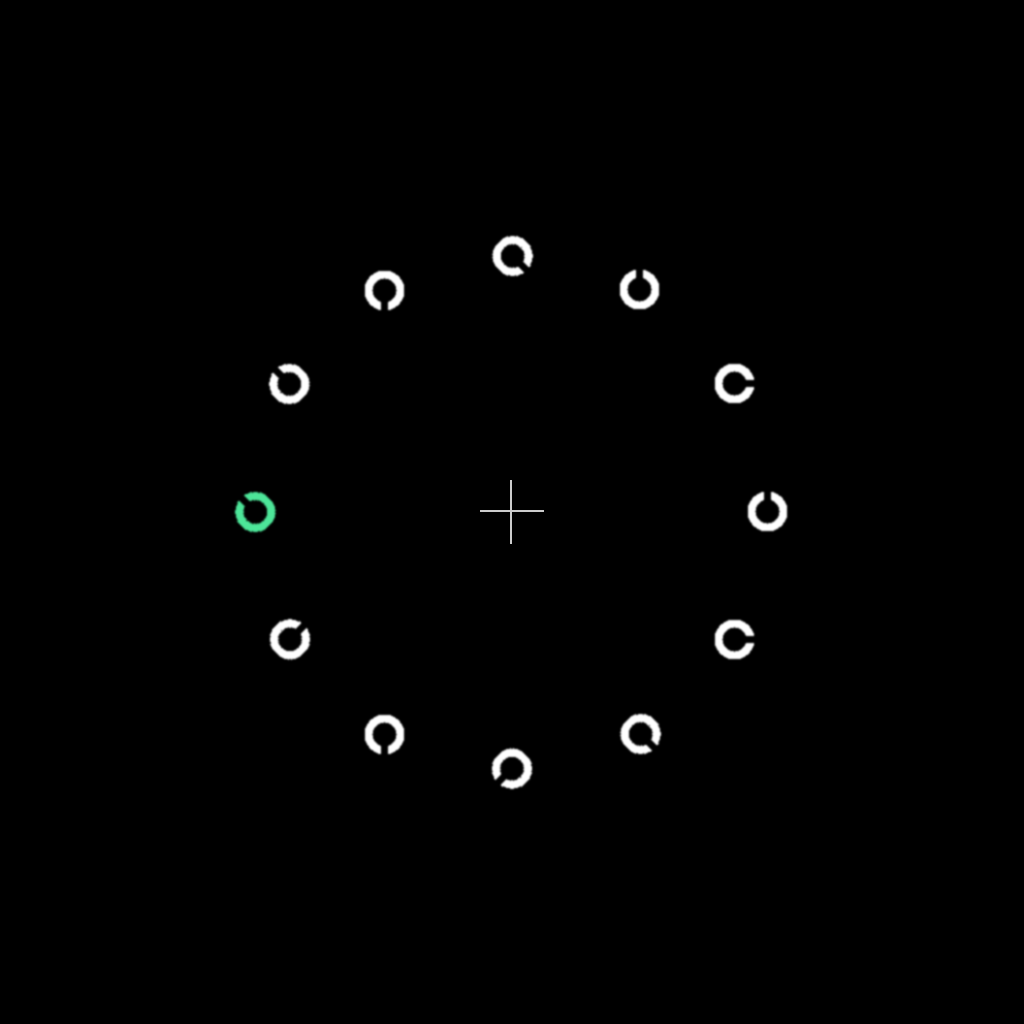
\includegraphics[width=6cm]{figs/exStimExp1.png}
\caption{Example stimulus from Experiment 1. Before the stimulus is shown, the observer is shown a green Landolt C. Their task is to decide if the green C in the stimulus matches the orientation of the previously presented C.}
\label{fig:exp1stimulus}
\end{figure}

\subsubsection{Procedure}
The first block of trials was pre-empted by a set of ten practice trials. The practice trials included the visual search condition only. There were then four blocks of 30 trials (15 for each condition). Each trial began with the presentation of a fixation cross followed by the presentation of a green Landolt C (the cue stimuli). The search array was then presented in the visual search condition. In the visualise search condition the cue stimuli was followed by instructions to 'visualise search' before the presentation of a further fixation cross. 
The orientation of the cued target, the location of the target within the search array and whether the target was present of absent was randomised for each trial

\subsection{Planned Analysis}

We plan to carry out the analysis in several different ways. Firstly, we will repeat the analysis from \cite{reinhart2015} in which the median reaction time for trial 1,2 and 3 within a (normal) run is compared to the median reaction time for trial 3 in a visualise-run. A one-tailed paired $t$-test will be used for this comparison. 

Additionally, we will also analyse the data in more detail using a linear mixed-effect model (\texttt{lme4} \citep{bates2015, R}), following the guidelines on model design given by \cite{barr2013} This allows us to include trial-to-trial variation in the analysis rather than using aggregate statistics. As the distribution of reaction times is expected to be skewed, we use log reaction times in the analysis. We will treat \textit{trial number} (within run) as a numerical factor, and will investigate non-linear regression if there is the asymptote is having a large effect on the data. However, given the results presented by \cite{reinhart2015}, a linear model should suffice. We will follow the model simplification procedure put forward by \cite[chapter 9]{crawley2012}. $p$-values will be obtained via the \texttt{Anova} function from the \texttt{car} package \citep{fox2011}.

Finally, we will also compare the visualisation effect to the effect of serial dependency. More specifically, we will investigate how reaction time varies on trial three depending on whether it preceded by two target present trials, two target absent trials, $\ldots$, or two visualise trials. This will be modelled using another linear mixed-effect model with a five-level factor describing the previous two trials, and a two-level factor for whether trial three is a target absent or present trial.

\subsection{Results and Discussion}


\centering
\textit{blank}

%%%%%%%%%%%%%%%%%%%%%%%%%%%%%%%%%%%%%%%%%%%%%%%%%%%%%
\section{Experiment 2}
\label{sec:exp2}
%%%%%%%%%%%%%%%%%%%%%%%%%%%%%%%%%%%%%%%%%%%%%%%%%%%%%

The aim of experiment two is to investigate whether the effect reported by \cite{reinhart2015} applies to more standard visual search paradigms, or if it is specific to the target matching task they used in their original study. Hence, in this study we remove the colour cue from the stimuli and change the observer's task from `does the green item match the target template?' to `is the target present of absent in this stimulus?.' This study will only be run if we successfully replicate the visualisation effect in Experiment 1. 

\subsection{Methods}

Identical to Experiment 1, except the colour cue has been removed and participants are simply reporting whether the target is present or absent. As this task is slightly more difficult, stimulus display time has been increased from 2000ms to 5000ms. 

\subsection{Results and Discussion}


\centering
\textit{blank}

%%%%%%%%%%%%%%%%%%%%%%%%%%%%%%%%%%%%%%%%%%%%%%%%%%%%%
\section{General Discussion}
\label{sec:discussion}
%%%%%%%%%%%%%%%%%%%%%%%%%%%%%%%%%%%%%%%%%%%%%%%%%%%%%

\centering
\textit{blank}

\begin{acknowledgements}
Thank you to Courtney Barr. 
\end{acknowledgements}

% BibTeX users please use one of
% \bibliographystyle{spbasic}      % basic style, author-year citations
%\bibliographystyle{spmpsci}      % mathematics and physical sciences
%\bibliographystyle{spphys}       % APS-like style for physics

\bibliographystyle{plainnat}
\bibliography{literature}

\end{document}
% end of file template.tex

